\subsection{Towards a wearable device (Q3)}
\label{sec:res-device}

\subsubsection{Which sensors}

With person scaling and one forest per limb (Table~\ref{tab:sensors}), two foot IMUs are the best device: 92.3\,\% (87--96).
Adding the thigh and shank IMUs does not help (all six: 91.2\,\%). Two thigh IMUs give 80.4\,\% and two shank IMUs 79.4\,\%,
each mainly through one limb. A single foot IMU on one leg, which is sometimes the leading and sometimes the trailing foot,
gives 83--91\,\% (Table~\ref{tab:onesensor}). Because the leading leg is not fixed (45\,\% dominant), a sensor on each foot is
the safe design. Figure~\ref{fig:device} summarises this subsection.

\begin{table}[htbp]
\centering
\caption{Height accuracy by sensor site (person scaling, random forest; leading limb, trailing limb, soft vote of both).}
\label{tab:sensors}
\begin{adjustbox}{max width=\textwidth}
{\footnotesize
\begin{tabular}{p{4.6cm}rrr}
\toprule
\textbf{sensors} & \textbf{leading leg only} & \textbf{trailing leg only} & \textbf{both legs (soft vote)} \\
\midrule
thigh IMU & 77.4\% (67--85) & 44.2\% (35--53) & 80.4\% (72--88) \\
shank IMU & 49.8\% (41--56) & 78.2\% (68--86) & 79.4\% (70--87) \\
foot IMU & 88.8\% (85--93) & 85.0\% (77--91) & 92.3\% (87--96) \\
thigh + shank + foot (3 per leg) & 87.7\% (83--92) & 86.6\% (79--92) & 91.2\% (86--96) \\
\bottomrule
\end{tabular}
}
\end{adjustbox}

\end{table}

\begin{table}[htbp]
\centering
\caption{One sensor on one leg only (it is the leading leg in some crossings and the trailing leg in others).}
\label{tab:onesensor}
\begin{adjustbox}{max width=\textwidth}
{\footnotesize
\begin{tabular}{lrr}
\toprule
\textbf{sensor} & \textbf{right leg} & \textbf{left leg} \\
\midrule
thigh IMU & 58.1\% (46--69) & 63.5\% (54--73) \\
shank IMU & 62.6\% (50--72) & 65.5\% (57--73) \\
foot IMU & 82.9\% (76--90) & 90.9\% (88--94) \\
\bottomrule
\end{tabular}
}
\end{adjustbox}

\end{table}

\subsubsection{How much calibration a new user needs}

Table~\ref{tab:calibration} compares what the two-foot device needs from a new user. Without information on the person
(population or level-walk offset) the accuracy is 56--58\,\%; the clearance-shape features alone give 72.8\,\%. The
physics-informed offset model needs only \emph{one} labelled crossing of any height to reach 80.3\,\%, and one labelled crossing per
height for 87.8\,\%. Without any label, person scaling from 10--15 random crossings gives 81--85\,\% and from a whole session
92.3\,\%. The ``first $n$'' rows follow the study's blocked order, in which the first crossings cover only one or two obstacles,
so they are pessimistic (Section~\ref{sec:res-realworld}).

\begin{table}[htbp]
\centering
\caption{Calibration options for a new user with two foot IMUs.}
\label{tab:calibration}
\begin{adjustbox}{max width=\textwidth}
{\footnotesize
\begin{tabular}{p{7.6cm}p{4.4cm}r}
\toprule
\textbf{approach} & \textbf{what the device needs from the new user} & \textbf{accuracy} \\
\midrule
generic model (logistic), level-walk scaling & a short normal walk & 56.4\% \\
generic model (forest), level-walk scaling & a short normal walk & 57.5\% \\
generic model (logistic), lead-foot clearance-shape features only, level-walk scaling & a short normal walk & 72.8\% \\
offset model, population offset & nothing & 56.3\% \\
offset model, offset from the level walk & a short normal walk & 56.9\% \\
offset model, 1 labelled crossing of ANY height & 1 crossing with known height & 80.3\% \\
offset model, 1 labelled crossing per height & 3 crossings with known heights & 87.8\% \\
offset model, unlabelled crossings (mixture, spacing fixed by physics) & the session's crossings, no labels & 77.0\% \\
weighted logistic, 1 labelled crossing per height & 3 crossings with known heights & 74.6\% \\
person scaling from the first 5 crossings (forest) & 5 unlabelled crossings & 60.4\% \\
person scaling from the first 10 crossings (forest) & 10 unlabelled crossings & 66.5\% \\
person scaling from the first 15 crossings (forest) & 15 unlabelled crossings & 67.9\% \\
person scaling from the random 5 crossings (forest) & 5 unlabelled crossings & 71.4\% \\
person scaling from the random 10 crossings (forest) & 10 unlabelled crossings & 81.2\% \\
person scaling from the random 15 crossings (forest) & 15 unlabelled crossings & 85.1\% \\
person scaling from all crossings (forest) & all the session's crossings, no labels & 92.3\% \\
\bottomrule
\end{tabular}
}
\end{adjustbox}

\end{table}

\subsubsection{Answering only when confident, and more training data}

If the device answers only when its top-class probability exceeds a threshold, its accuracy on the answered crossings rises
from 92.3\,\% to 96.6\,\% (threshold 0.6, 79\,\% answered) and 98.3\,\% (0.8, 46\,\% answered; Table~\ref{tab:confidence}). A
model trained on only two or three participants already reaches 88--89\,\% (Table~\ref{tab:learning}): more participants add
little; the remaining errors come from person-to-person differences, which calibration addresses.

\begin{table}[htbp]
\centering
\begin{minipage}{0.46\textwidth}
\centering
\caption{Answering only above a probability threshold.}
\label{tab:confidence}
\begin{adjustbox}{max width=\textwidth}
{\footnotesize
\begin{tabular}{rrr}
\toprule
\textbf{answer when top probability $\geq$} & \textbf{crossings answered} & \textbf{accuracy on them} \\
\midrule
0.0 & 100\% & 92.3\% \\
0.5 & 94\% & 93.9\% \\
0.6 & 79\% & 96.6\% \\
0.7 & 67\% & 97.7\% \\
0.8 & 46\% & 98.3\% \\
\bottomrule
\end{tabular}
}
\end{adjustbox}

\end{minipage}\hfill
\begin{minipage}{0.46\textwidth}
\centering
\caption{Learning curve: training participants vs accuracy (10 random draws).}
\label{tab:learning}
\begin{adjustbox}{max width=\textwidth}
{\footnotesize
\begin{tabular}{rrr}
\toprule
\textbf{training participants} & \textbf{accuracy (mean)} & \textbf{range over draws} \\
\midrule
2 & 88.5\% & 85.8--90.4\% \\
3 & 89.1\% & 87.3--91.5\% \\
4 & 90.3\% & 89.1--91.9\% \\
5 & 90.4\% & 88.8--92.3\% \\
6 & 90.4\% & 88.8--91.6\% \\
7 & 91.4\% & 90.4--92.3\% \\
8 & 91.4\% & 90.4--92.3\% \\
9 & 92.3\% & 92.3--92.3\% \\
\bottomrule
\end{tabular}
}
\end{adjustbox}

\end{minipage}
\end{table}

\begin{figure}[htbp]
\centering
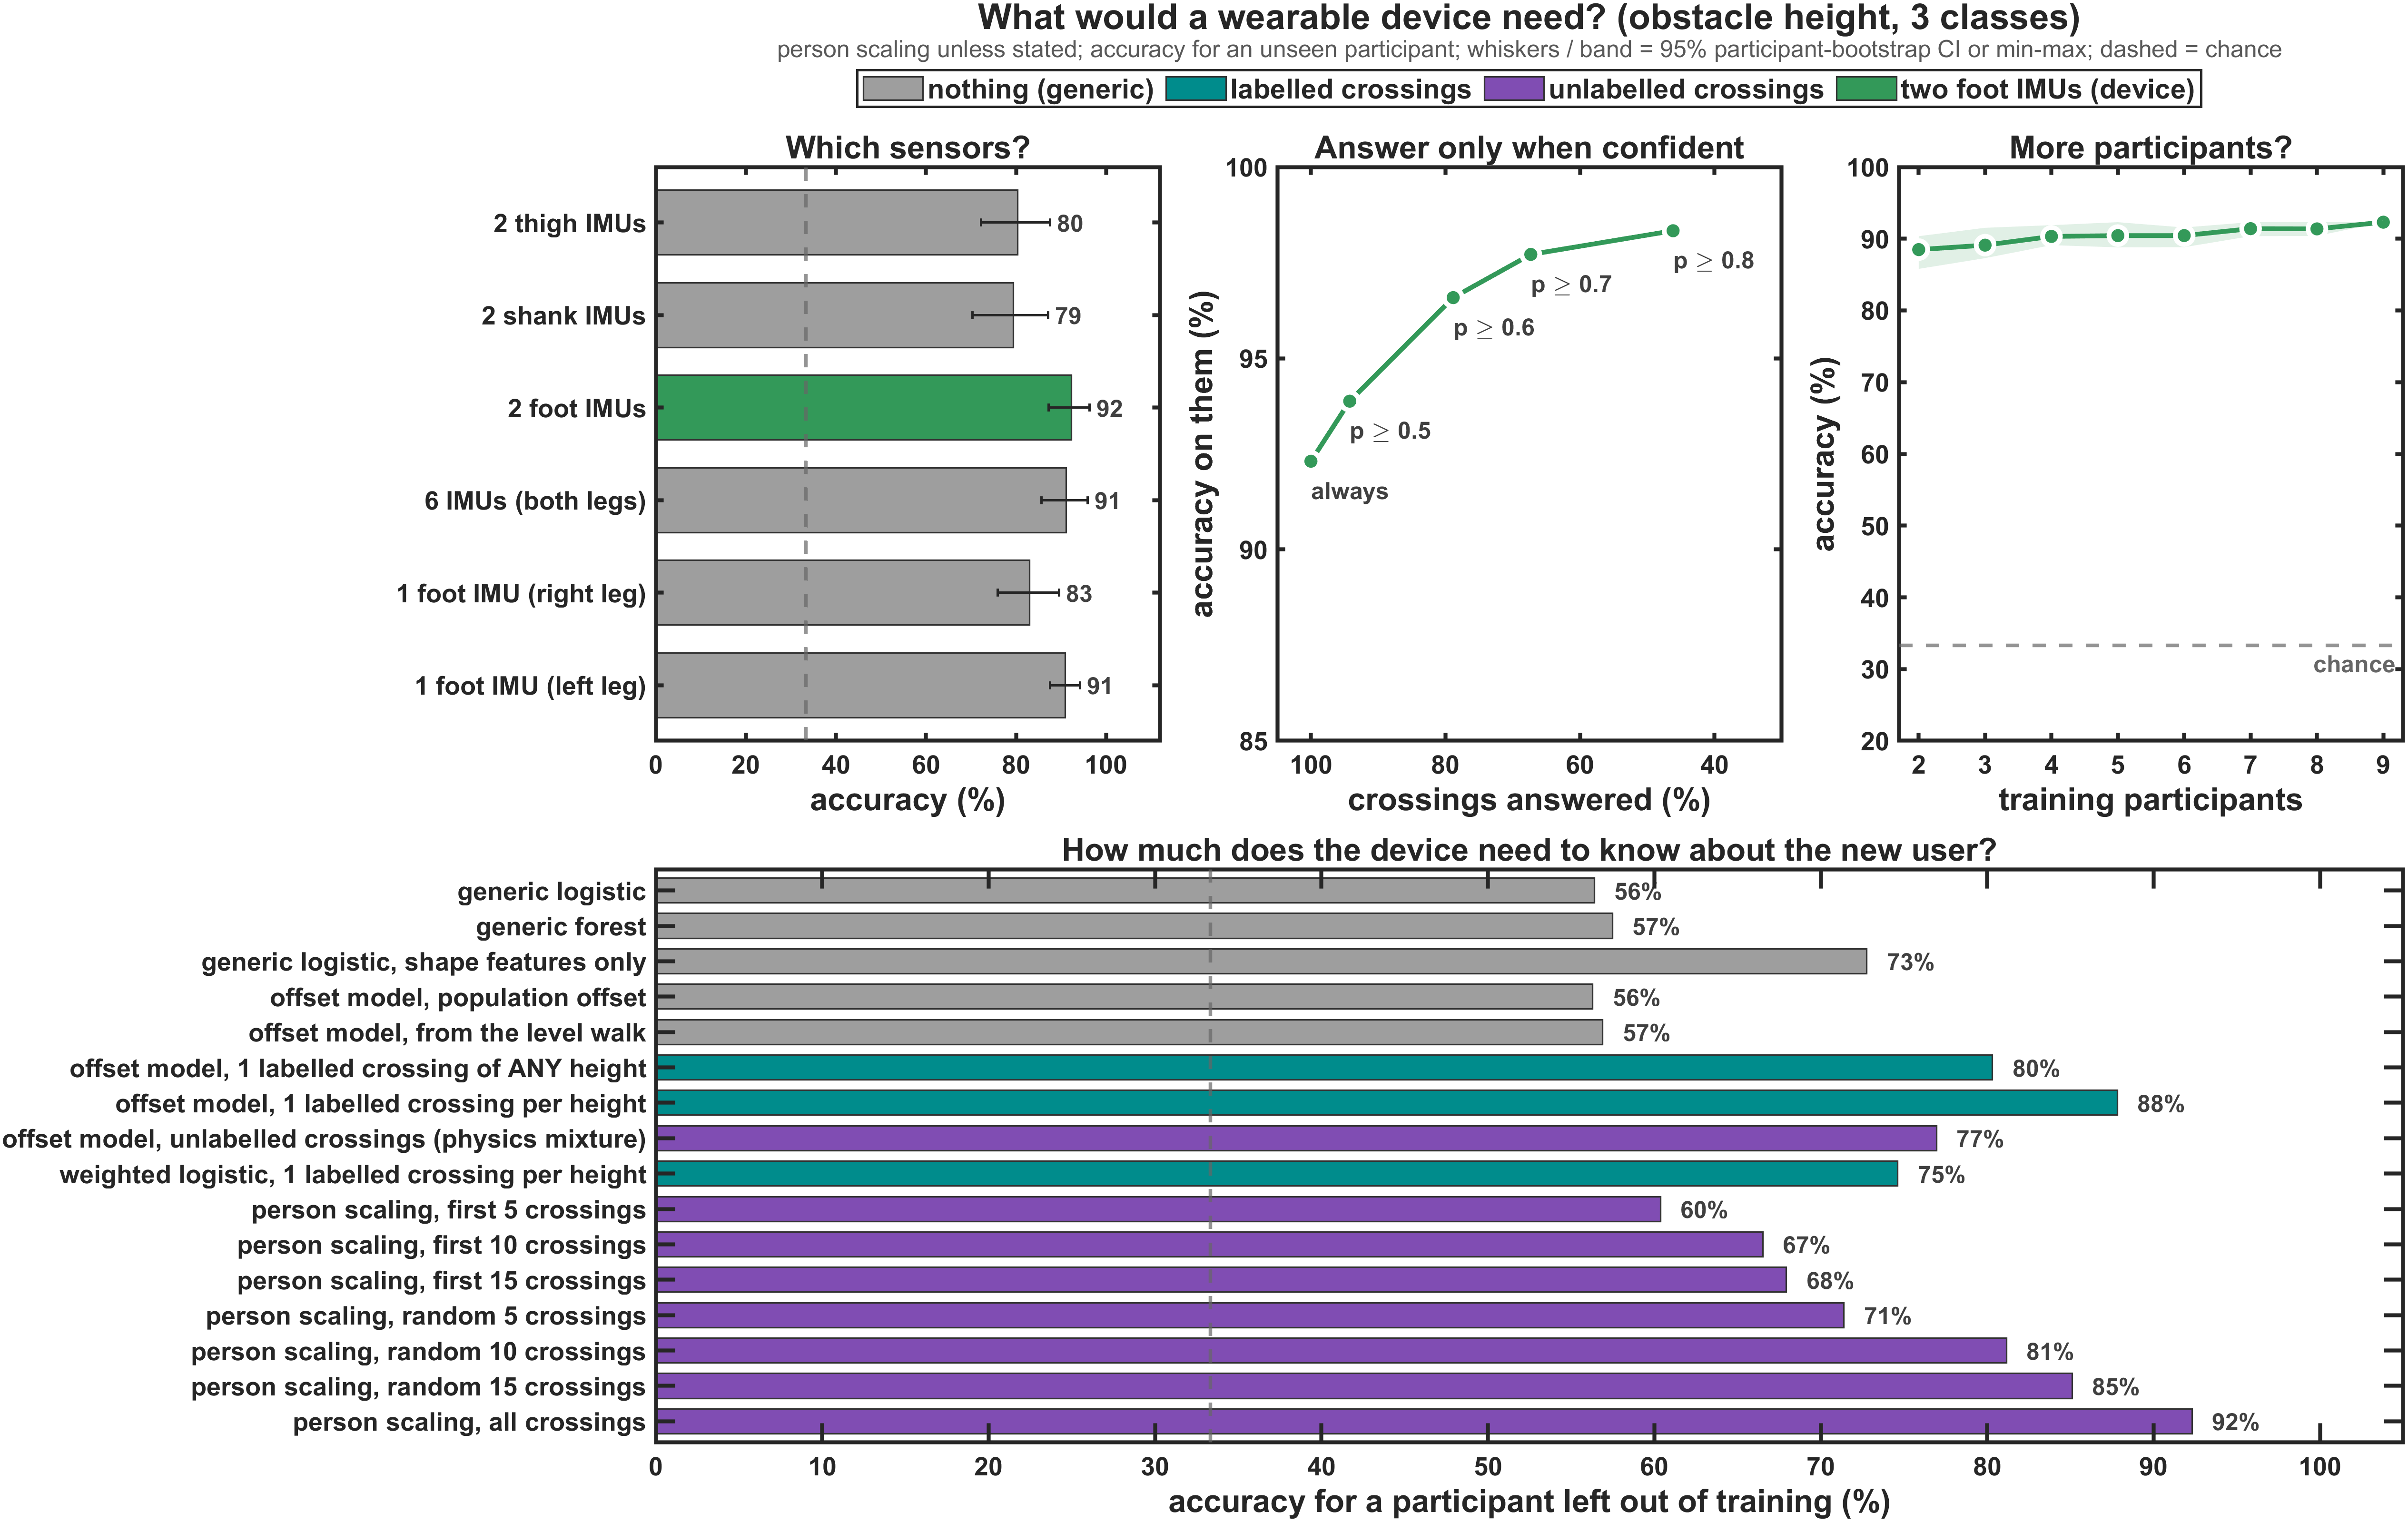
\includegraphics[width=\textwidth]{fig_device.png}
\caption{Device questions. Top: sensor sites (95\,\% CI; green = the two foot IMUs), accuracy against the share of crossings
answered when the device answers only above a probability threshold, and accuracy against the number of training participants
(band = min--max over the draws). Bottom: calibration options (grey = nothing about the new user, teal = labelled crossings,
purple = unlabelled crossings).}
\label{fig:device}
\end{figure}

\subsubsection{No camera: the end-to-end pipeline}

The pipeline that uses only the Dot (Table~\ref{tab:streamdetect}, Table~\ref{tab:streame2e}, Figure~\ref{fig:stream}) scans all
7250 strides of the sessions. It finds the obstacle-crossing strides with 98.7\,\% recall and 97.2\,\% precision, pairs them
into crossings with the right leading and trailing strides for 95.2\,\% of the crossings, and gives the right height for
90.7\,\% of the found crossings: 86.3\,\% of the crossings are fully correct (83.5\,\% when the 10 crossings without a valid
toe-off are counted as missed). Scaling the height features with the person's normal walking instead of their detected
crossings gives only 52.9\,\%: the personal scaling must come from crossings.

\begin{table}[htbp]
\centering
\caption{Finding the crossing strides among all strides of the session.}
\label{tab:streamdetect}
\begin{adjustbox}{max width=\textwidth}
{\footnotesize
\begin{tabular}{llrrr}
\toprule
\textbf{features} & \textbf{model} & \textbf{balanced accuracy} & \textbf{recall (crossings found)} & \textbf{precision (detections that are crossings)} \\
\midrule
raw & logistic & 93.8\% & 88.1\% & 94.8\% \\
raw & random forest & 99.2\% & 98.8\% & 95.9\% \\
scaled to own walking & logistic & 94.6\% & 89.6\% & 94.5\% \\
scaled to own walking & random forest & 99.2\% & 98.7\% & 97.2\% \\
\bottomrule
\end{tabular}
}
\end{adjustbox}

\end{table}

\begin{table}[htbp]
\centering
\caption{End to end: detect, pair (first foot = leading), classify the height.}
\label{tab:streame2e}
\begin{adjustbox}{max width=\textwidth}
{\footnotesize
\begin{tabular}{lrrrrr}
\toprule
\textbf{height scaling} & \textbf{crossings found} & \textbf{lead + trail strides right} & \textbf{height right (when found)} & \textbf{ALL correct} & \textbf{false crossings (per person)} \\
\midrule
crossing-scaled & 95.2\% & 95.2\% & 90.7\% & \textbf{86.3\%} & 1.4 \\
walking-scaled & 95.2\% & 95.2\% & 55.6\% & \textbf{52.9\%} & 1.4 \\
\bottomrule
\end{tabular}
}
\end{adjustbox}

\end{table}

\begin{figure}[htbp]
\centering
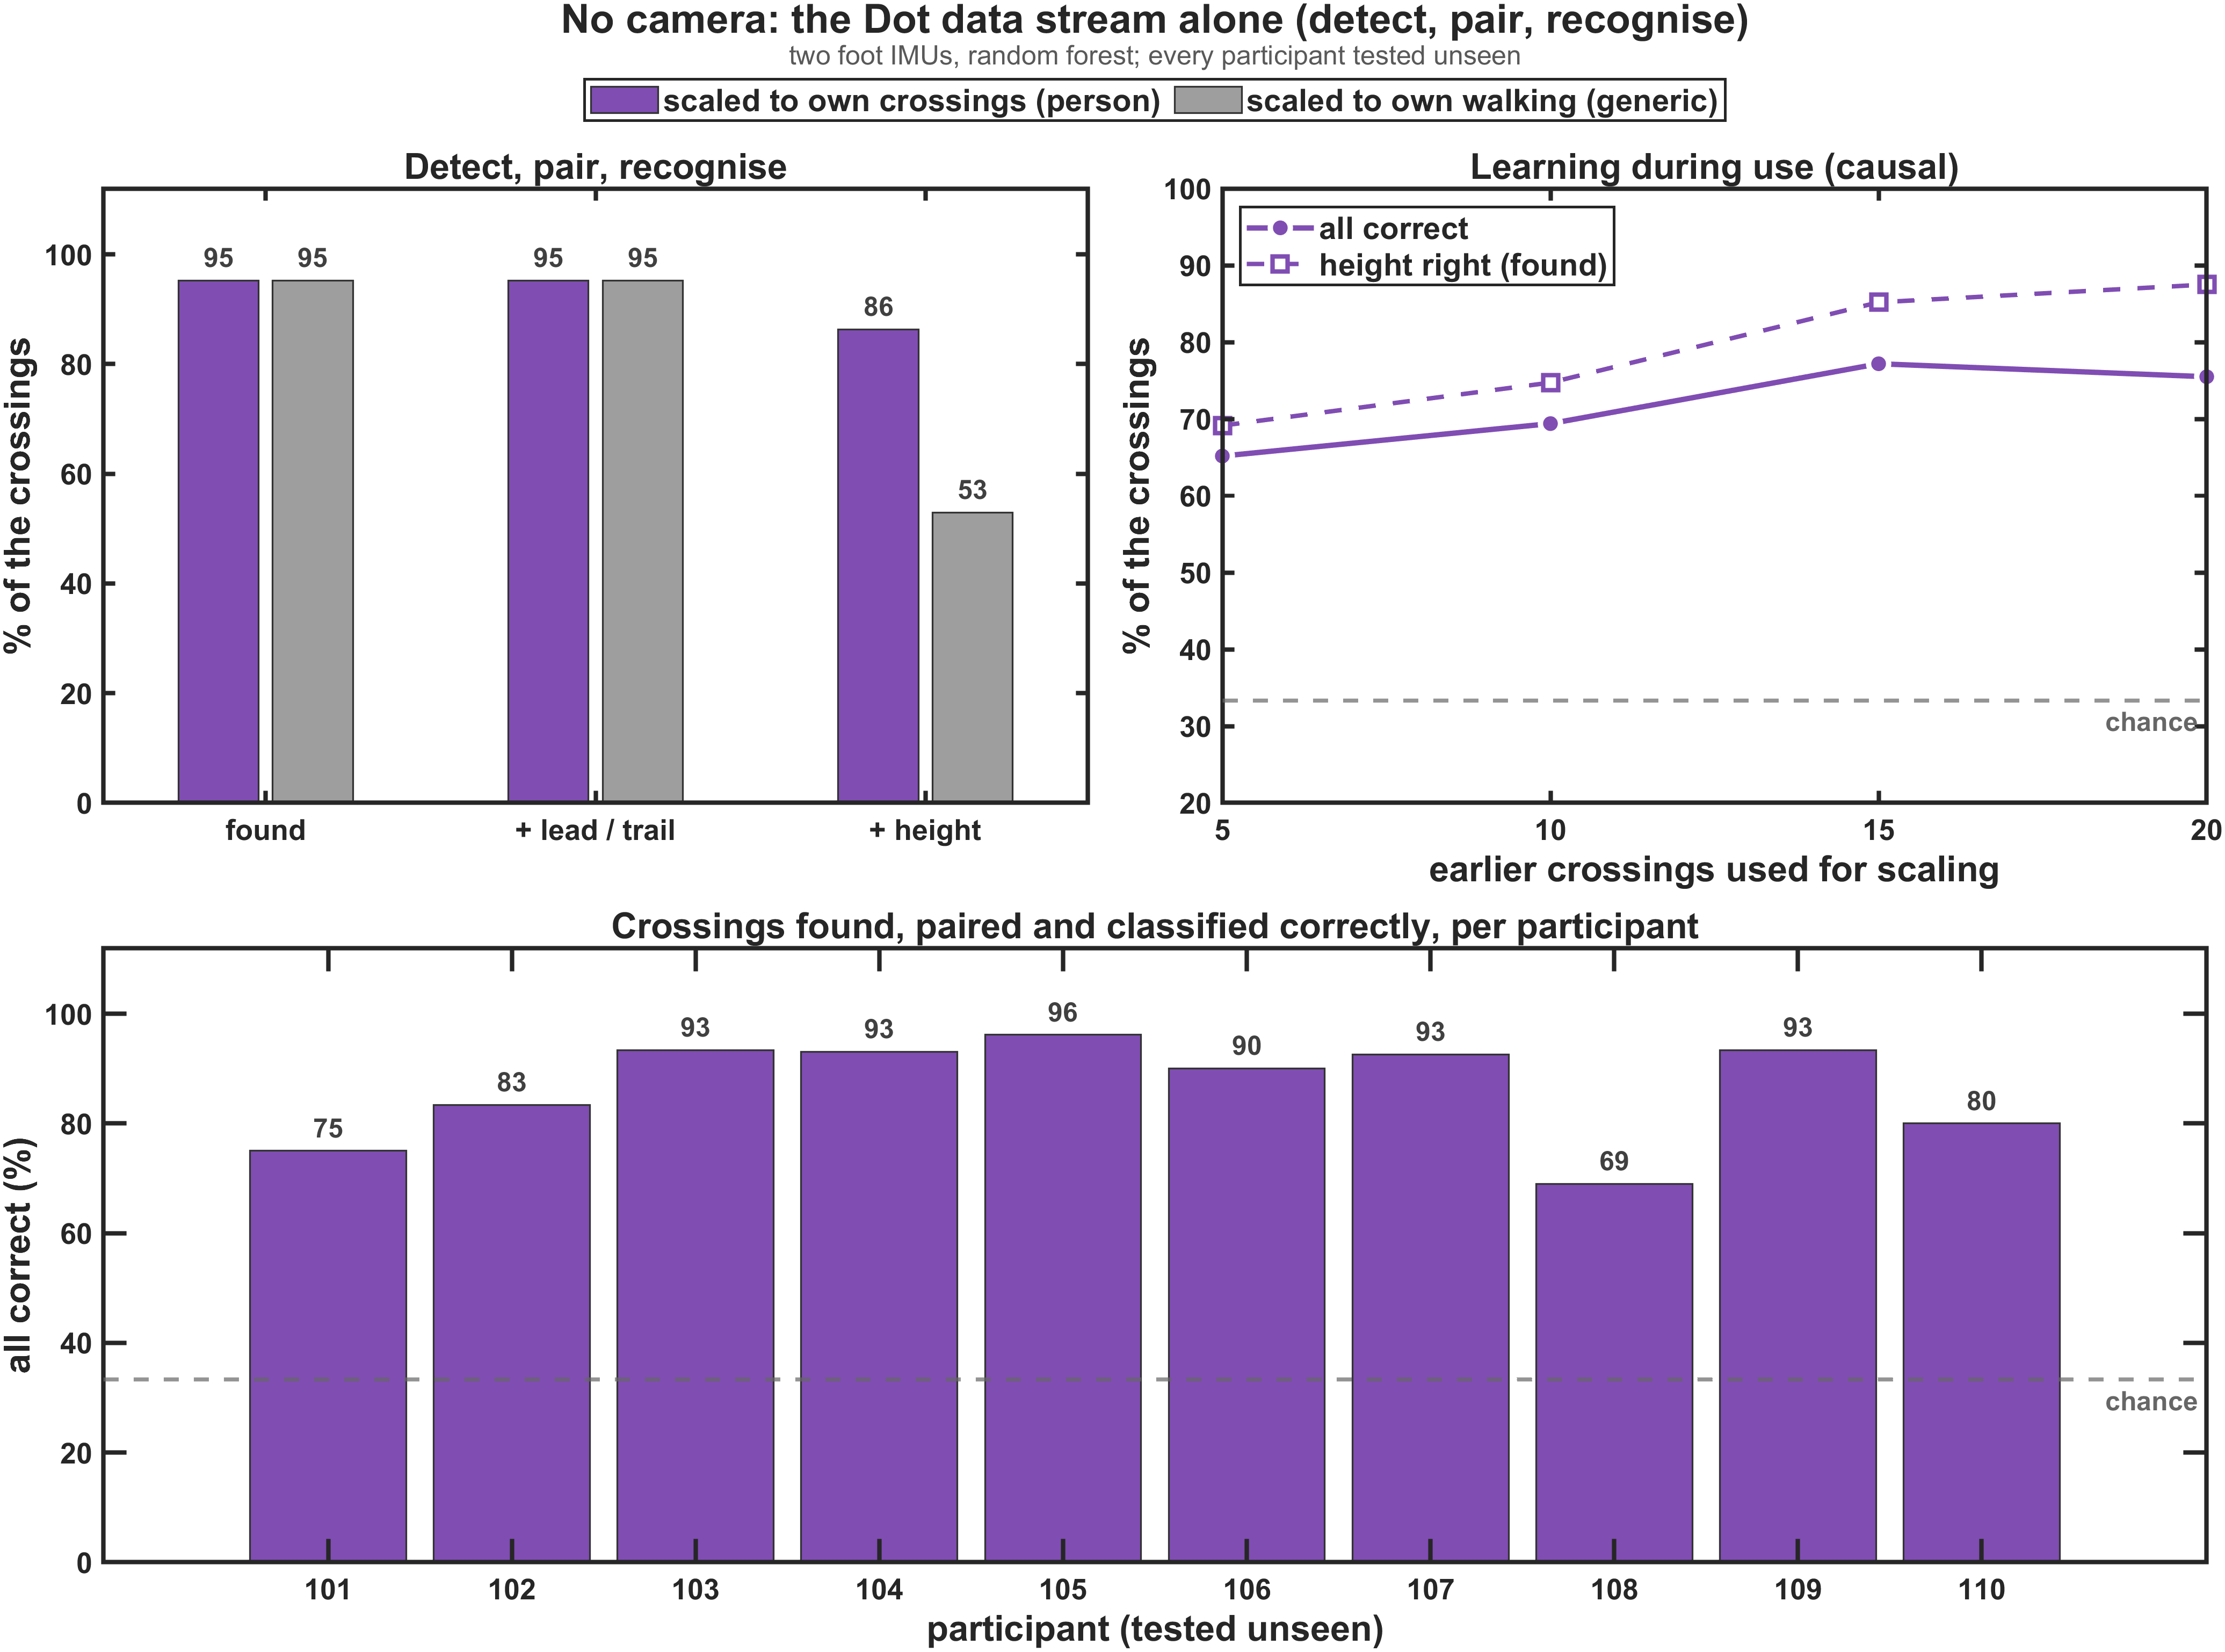
\includegraphics[width=\textwidth]{fig_stream.png}
\caption{Camera-free pipeline. Top left: share of the crossings found, also paired correctly (leading / trailing) and also
classified correctly, with the features scaled to the person's own crossings (purple) or own walking (grey). Top right: learning
during use (each crossing scaled with the earlier detected crossings only). Bottom: all-correct crossings per participant.}
\label{fig:stream}
\end{figure}

\subsubsection{A realistic session: obstacles in mixed order}
\label{sec:res-realworld}

The study ran the obstacles in blocks, but in daily life they come mixed. Each participant's crossings were shuffled 30 times and
the device worked causally: generic model for the first 5 (or 10) crossings, then person scaling learned from the crossings
already walked, without labels (Table~\ref{tab:mixed}, Figure~\ref{fig:realworld}). In mixed order the accuracy grows steadily
from 72\,\% (crossings 1--5) to 79\,\% (6--15) and 90\,\% from crossing 16 on. In the blocked study order the early history
covers only one or two obstacles, the person scaling is biased, and the accuracy collapses for crossings 6--15 before catching up.
The study's blocked-order ``learning during use'' numbers are therefore pessimistic for real use.

\begin{table}[htbp]
\centering
\caption{Accuracy by crossing number in a session, mixed (mean of 30 random orders) vs the real blocked order; generic model until
the switch, then causal person scaling.}
\label{tab:mixed}
\begin{adjustbox}{max width=\textwidth}
{\footnotesize
\begin{tabular}{llrrrrrr}
\toprule
\textbf{order} & \textbf{switch after} & \textbf{crossings 1--5} & \textbf{6--10} & \textbf{11--15} & \textbf{16--20} & \textbf{21+} & \textbf{all} \\
\midrule
mixed & 5 crossings & 71.9\% & 75.1\% & 82.9\% & 87.9\% & 91.3\% & 82.2\% \\
blocked & 5 crossings & 70.0\% & 46.0\% & 56.0\% & 81.2\% & 90.3\% & 69.6\% \\
mixed & 10 crossings & 71.9\% & 73.3\% & 82.9\% & 87.9\% & 91.3\% & 81.9\% \\
blocked & 10 crossings & 70.0\% & 68.0\% & 56.0\% & 81.2\% & 90.3\% & 73.8\% \\
\bottomrule
\end{tabular}
}
\end{adjustbox}

\end{table}

\subsubsection{A virtual real-time cue}
\label{sec:res-cue}

A real-time device must (a) notice the crossing and (b) decide the height while there is still time to cue the trailing limb.
(a) Over all 7250 strides of the sessions, online features available at the foot apex detect 99.0\,\% of the leading-limb
crossing strides, with about 3 false detections per session of about 725 strides. (b) The height is then predicted from the
leading-limb data available at the leading-foot apex (450\,ms before the trailing toe lift-off) or at its landing (200\,ms
before), with causal person scaling (Table~\ref{tab:cue}). In a mixed session about 71\,\% of the crossings get a correct cue at
the apex (76\,\% at landing); after 15 crossings 76\,\% (83\,\%). Answering only above a probability of 0.6 makes 79--82\,\% of
the given cues right but withholds 25--30\,\% of them. The real-time cue is less accurate than the after-the-fact recognition
(about 92\,\%) because only the leading limb has crossed when the cue must be sent.

\begin{table}[htbp]
\centering
\caption{Virtual real-time cue: outcome per crossing (correct / wrong / no cue), share of the given cues that are right, and the
correct cues after 15 crossings. Time left = median time to the trailing toe lift-off.}
\label{tab:cue}
\begin{adjustbox}{max width=\textwidth}
{\scriptsize
\begin{tabular}{lrlrrrrrr}
\toprule
\textbf{cue at} & \textbf{time left} & \textbf{order} & \textbf{threshold} & \textbf{correct cue} & \textbf{wrong cue} & \textbf{no cue (missed or unsure)} & \textbf{cues that are right} & \textbf{correct cue after 15 crossings} \\
\midrule
lead foot apex & 450 ms & mixed & 0.0 & 71.2\% & 27.7\% & 1.2\% & 72.0\% & 76.3\% \\
lead foot apex & 450 ms & mixed & 0.6 & 55.6\% & 14.7\% & 29.8\% & 79.1\% & 63.3\% \\
lead foot apex & 450 ms & blocked & 0.0 & 58.8\% & 40.0\% & 1.2\% & 59.5\% & 75.5\% \\
lead foot apex & 450 ms & blocked & 0.6 & 49.6\% & 23.5\% & 26.9\% & 67.9\% & 65.5\% \\
lead landing & 200 ms & mixed & 0.0 & 75.8\% & 23.1\% & 1.2\% & 76.6\% & 83.2\% \\
lead landing & 200 ms & mixed & 0.6 & 61.2\% & 13.7\% & 25.1\% & 81.7\% & 69.1\% \\
lead landing & 200 ms & blocked & 0.0 & 65.0\% & 33.8\% & 1.2\% & 65.8\% & 80.9\% \\
lead landing & 200 ms & blocked & 0.6 & 54.6\% & 25.0\% & 20.4\% & 68.6\% & 73.6\% \\
\bottomrule
\end{tabular}
}
\end{adjustbox}

\end{table}

\subsubsection{Why some participants are harder}

Once the device is scaled to the person, its errors follow how consistently that person lifts the \emph{trailing} foot for a given
height (Table~\ref{tab:dprime}): the person-scaled accuracy correlates with the trailing-foot separability $d'$ ($r = 0.77$,
leading $d'$: $r = 0.25$). The weakest participant (108, 73\,\%) has by far the least consistent trailing lift ($d' = 0.9$). The
generic model behaves differently ($r = -0.66$ with the trailing $d'$): its errors come from how far a person's personal margin
is from the group, which person scaling removes. With ten participants these correlations are indicative.

\begin{table}[htbp]
\centering
\caption{Per participant: separability of the heights in the leading and trailing foot lift ($d'$), the leading-foot lift SD within
a height and its slope, and the accuracy with person scaling and with the generic model.}
\label{tab:dprime}
\begin{adjustbox}{max width=\textwidth}
{\footnotesize
\begin{tabular}{lrrrrrr}
\toprule
\textbf{participant} & \textbf{lead lift $d'$} & \textbf{trail lift $d'$} & \textbf{lead lift SD within height (mm)} & \textbf{lead slope (mm/cm)} & \textbf{accuracy, person-scaled} & \textbf{accuracy, generic} \\
\midrule
101 & 3.0 & 2.1 & 33 & 11.1 & 94\% & 83\% \\
102 & 2.5 & 2.7 & 45 & 11.2 & 90\% & 63\% \\
103 & 3.7 & 3.6 & 22 & 8.6 & 100\% & 72\% \\
104 & 3.6 & 3.2 & 20 & 8.5 & 96\% & 54\% \\
105 & 4.7 & 2.2 & 19 & 10.2 & 96\% & 84\% \\
106 & 1.2 & 3.4 & 92 & 10.0 & 97\% & 69\% \\
107 & 2.8 & 2.5 & 37 & 10.8 & 85\% & 85\% \\
108 & 2.7 & 0.9 & 29 & 8.8 & 73\% & 85\% \\
109 & 3.5 & 4.5 & 28 & 10.7 & 96\% & 50\% \\
110 & 3.0 & 3.4 & 29 & 10.7 & 96\% & 83\% \\
\bottomrule
\end{tabular}
}
\end{adjustbox}

\end{table}

\begin{figure}[htbp]
\centering
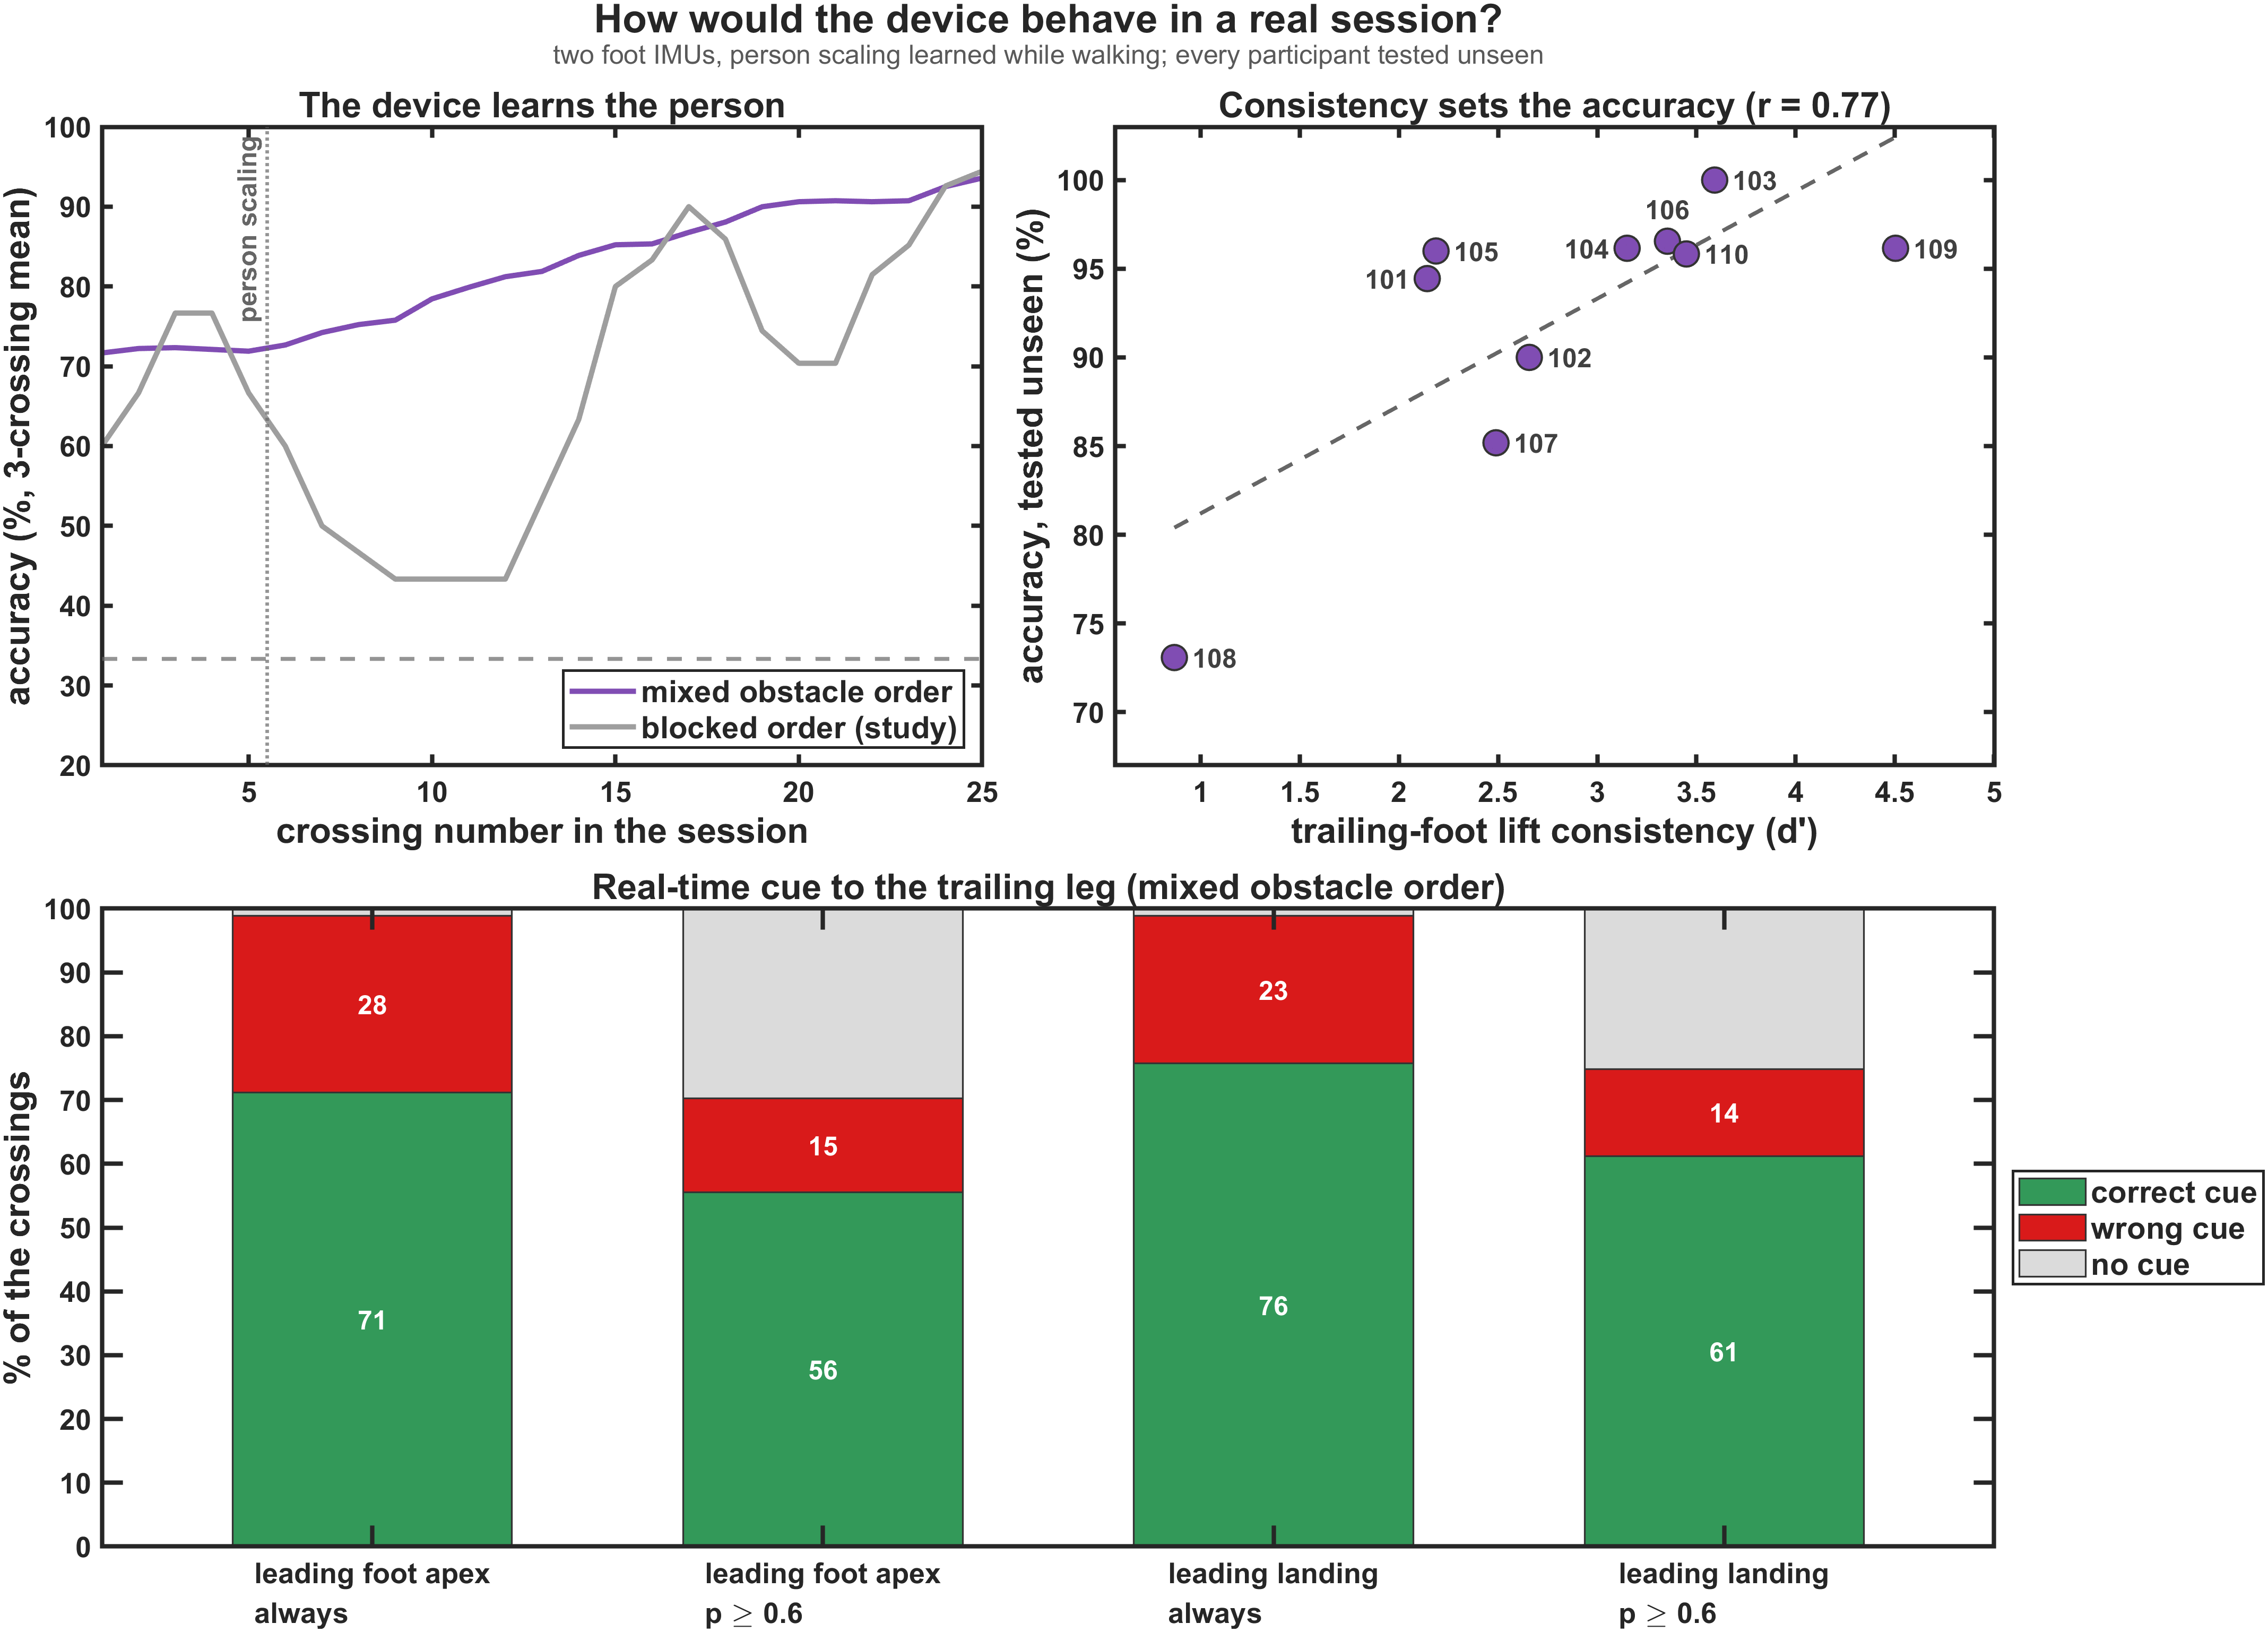
\includegraphics[width=\textwidth]{fig_realworld.png}
\caption{Real-world questions. Top left: accuracy by crossing number in a mixed vs blocked obstacle order (3-crossing moving
mean; dotted = start of person scaling; dashed = chance). Top right: person-scaled accuracy against the trailing-foot separability $d'$ per participant (dashed = least-squares line).
Bottom: outcome of the virtual real-time cue to the trailing leg for each cue moment and confidence threshold (green = correct,
red = wrong, grey = no cue).}
\label{fig:realworld}
\end{figure}

